%-------------------------------------------------------------------------------
\documentclass[a4paper, 12pt] {article}
%-------------------------------------------------------------------------------
\usepackage[brazil]{babel}
\usepackage[utf8]{inputenc}
\usepackage{graphicx}
\usepackage[none]{hyphenat}
\usepackage{indentfirst}
\usepackage{setspace}
\usepackage{comment}
\usepackage{amsmath}
\usepackage{amssymb}
%-------------------------------------------------------------------------------
\newcommand{\p}{$\bullet$}
%-------------------------------------------------------------------------------
\addtolength{\hoffset}{-1.5cm}
\addtolength{\voffset}{-2.0cm}
\addtolength{\textwidth}{3.0cm}
\addtolength{\textheight}{4.1cm}
%-------------------------------------------------------------------------------
\sloppy
%------------------------------------------------------------------------------
\begin{document}

\thispagestyle{empty}
\begin{center}

\vskip 2.2cm

\Large{Título: Algoritmos Multi-BSP para o problema da subsoma de tamanho máximo
3D}

\vskip 1.5cm

\Large{Projeto de Pesquisa}

\vskip 1.5cm

\Large{Projeto de Pesquisa apresentado como exigência da primeira fase do
processo seletivo para ingresso no programa de Doutorado em Computação promovido entre a Universidade Federal de Mato Grosso Sul e a 
Universidade Federal de Goiás.}

\vskip 2.5cm

\Large{Candidato: Rodrigo Gonçalves de Branco}

\vskip 2.0cm

%{\Large Orientador:}

\vskip 2.5cm

\large{Programa de Pós-Graduação em Ciência da Computação, nível de Doutorado,
da Faculdade de Computação da UFMS em associação com o Instituto de Informática da UFG}

\vskip 1.3cm

Campo Grande--MS, outubro de 2014

\end{center}

\clearpage
%-----------------------------------------------------------------
\onehalfspacing
%-------------------------------------------------------------------------------
\pagenumbering{arabic}

\section{Introdução}

O problema da subsoma de tamanho máximo pode ser definido como: dado um conjunto
de $n$ números reais, a subsoma de tamanho máximo é a maior soma contígua de
elementos, dentre todas as possíveis somas contíguas possíveis no conjunto
dado \cite{bentley2000programming}, tendo a Figura \ref{fig:maxsubsum} como
exemplo. Este problema pode ser encontrado em diversas áreas, como Biologia
Computacional, principalmente na localização de segmentos biológicos significantes e identificação de domínios
transmembranos em uma sequência de proteínas \cite{bae2007}. Jay Kadane
apresentou um algoritmo de complexidade $O(n)$ para resolver o problema descrito, utilizando 
programação dinâmica \cite{bentley2000programming}.

\begin{figure}[ht]
\centering
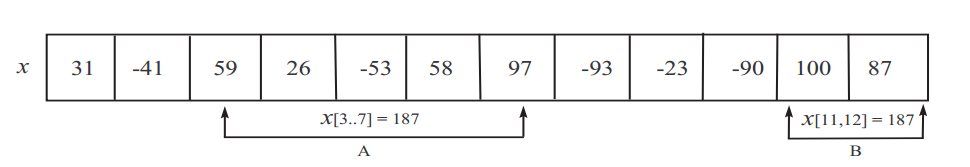
\includegraphics[width=\textwidth]{maxsubsum.png}
\caption{Vetor com 12 elementos, com duas subsomas de tamanho máximo.}
\label{fig:maxsubsum}
\end{figure}

Este problema pode ser estendido para duas dimensões. Dado uma matriz de $nxn$
números reais, a submatriz de soma máxima é a maior submatriz retangular cuja
soma de seus elementos apresenta a soma máxima, dentre todas as submatrizes
possíveis no conjunto de entrada apresentado. A Figura \ref{fig:maxsubarray}
apresenta um exemplo para este problema. A motivação para este problema pode ser
encontrada em áreas como visão computacional, identificando em imagens (sejam
elas de áreas médicas, de astronomia, termais, entre outras) as regiões de
interesse. A Figura {fig:brightest} apresenta um exemplo desta aplicação.

\begin{figure}[ht]
\centering
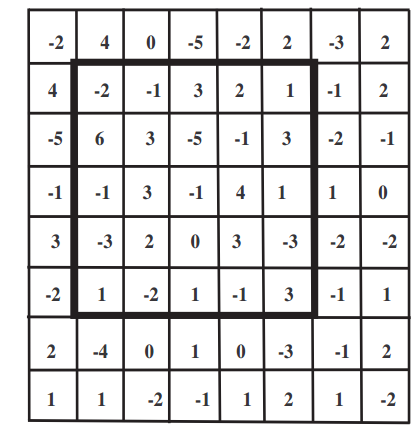
\includegraphics[width=.35\textwidth]{maxsubarray.png}
\caption{A região destacada é submatriz de soma máxima para a matriz
apresentada.}
\label{fig:maxsubarray}
\end{figure}

\begin{figure}[ht]
\centering
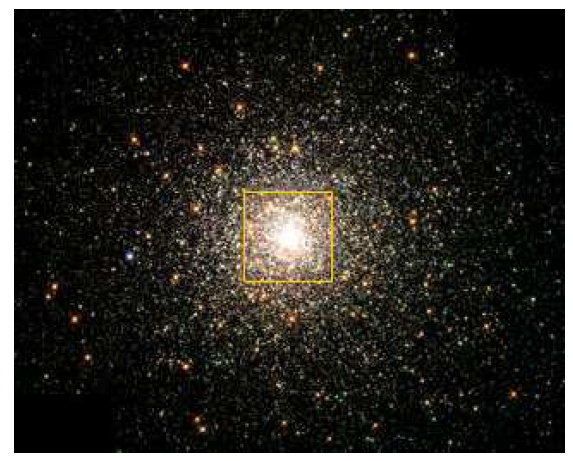
\includegraphics[width=.35\textwidth]{brightest.png}
\caption{Área mais brilhante em uma imagem de astronomia \cite{bae2007}.}
\label{fig:brightest}
\end{figure}

O algoritmo linear proposto por Kadane pode ser extendido para resolver a versão
2D. A matriz de entrada é substituida pela soma de prefixo de suas linhas, e com
essa nova matriz, a submatriz de soma máxima é então calculada da seguinte
forma: Para cada par de colunas possíveis (denominadas $Cgh$, tal que $1 <= g
<= h <= n$), o algoritmo linear de Kanade é usado para, naquela configuração de
colunas, encontrar a maior soma daquela configuração, delimitando portanto as linhas da matriz considerada. Assim, para
uma matriz com $nxn$ elementos, precisamos calcular $\frac{n(n-1)}{2} Cgh's$, e
cada um deles utiliza $O(n)$ passos para encontrar a submatriz de soma máxima
para aquela configuração, resultando assim em um algoritmo $O(n^3)$.

\subsection{Algoritmos Paralelos}

Em função do volume de dados das aplicações descritas anteriormente, as
versões apresentadas, executando em computadores tradicionais sequenciais, podem
não apresentar os resultados dentre de um período de tempo satisfatório. Por
esse motivo, diversos algoritmos paralelos, em diversos modelos, foram
apresentados para minimizar este problema.

\subsubsection{PRAM - Parallel Random Access Machine}

O modelo PRAM (\textit{Parallel Random Access Machine}) é uma máquina paralela
abstrata utilizada para modelar algoritmos paralelos teóricos que teriam um
comportamento previsível em termos assintóticos em computadores paralelos reais.
A vantagem do modelo PRAM é que ele ignora questões como comunicação entre os
processadores, permitindo que seu utilizador foque no potencial paralelismo do
algoritmo proposto. Os processadores não estão diretamente interligados entre
si, mas possuem acesso a uma memória global, onde podem trocar informações.

É possível encontrar algoritmos, tanto para o problema 1D quanto para o 2D,
descritos no modelo PRAM. Em \cite{journals/ppl/PerumallaD95}, para o problema
1D, um dos algoritmos  possui complexidade $O(log n)$, utilizando $O(\frac{n}{log
n})$ processadores. Para o problema 2D, o algoritmo apresentado também possui
complexidade $O(log n)$, utilizando $O(\frac{n^3}{log
n})$ processadores.

\subsubsection{BSP - Bulk Synchronous Parallel}

Leslie Valiant propôs o modelo BSP (\textit{Bulk Synchronous
Parallel}), com o objetivo de aproximar o
desenvolvimento de algoritmos paralelos para
arquiteturas reais \cite{Valiant:1990:BMP:79173.79181}. Este modelo não garante
comunicação e sincronização, e estes fatores devem ser considerados no projeto
de um algoritmo BSP. A Figura \ref{fig:bsp} apresenta um superpasso de um
algoritmo BSP.

\begin{figure}[ht]
\centering
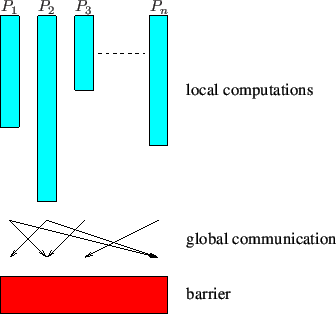
\includegraphics[width=.35\textwidth]{bsp.png}
\caption{Super passo BSP (computação local, comunicação e barreira de
sincronização)}
\label{fig:bsp}
\end{figure}

O modelo BSP pode ser combinado com o modelo CGM (\textit{Coarse Grained
Multicomputer}), este último apresentado por Dehne \textit{et al}
\cite{Dehne:1993:SPG:160985.161154}, em situações em que a entrada do problema é
muito maior que o número de processadores disponíveis. Um algoritmo CGM típico
consisten de uma sequência de rodadas, alternando entre etapas de computação e
comunicação separados por barreiras de comunicação.

Alves \textit{et al} apresentam algoritmos BSP/CGM tanto para o problema 1D
quanto para o problema 2D \cite{alves2004}. O problema 1D é resolvido com $p$
processadores, com tempo de computação local igual a  $O(\frac{n}{p})$ e $O(1)$
rodadas de comunicação. A solução do problema 2D difere do problema 1D no tempo
de computação local, pois este é igual a $O(\frac{n^3}{p})$.

\subsection{O problema 3D}

Os problemas 1D e 2D podem ser generalizados para $d$ dimensões, da seguinte
forma: dado um cubo $d-$dimensional com lado de tamanho $n$ de números reais,
encontre o sub$-d-$cubo que possui a maior soma de todos os sub$-d-$cubos
possíveis \cite{journals/ppl/PerumallaD95}. Usando a mesma estratégia da versão
2D descrita anteriormente, é possível descrever um algoritmo para resolver o
problema $n-$dimensional.





\section{Objetivos}

\section{Metodologia}

\section{Etapas e Cronograma}

\section{Resultados Esperados}

%-------------------------------------------------------------------------------
\bibliographystyle{unsrt}
\bibliography{proposta}
%-------------------------------------------------------------------------------
\end{document}
%-------------------------------------------------------------------------------